\headline{{\textbf{\Large\sffamily TWBC Workshops:}}\\
          {\textbf{\large\sffamily Critique of a Cork Bark Chinese Elm}}}
\label{2025-07-workshop}
\noindent
Our latest club gathering was a real treat, thanks to Tina Todd, who brought in a charming Chinese bark elm for critique. The little tree was a gift to her a couple of years ago, and after letting it grow freely for a while, Tina felt it was time to refine its direction --- so she turned to the club for advice.  

\vspace{-0.5em}
\medskip
The tree had plenty of potential, with healthy growth and an interesting structure, but Tina wasn't entirely sure how to develop it further. That's where the club's collective wisdom came into play! Members eagerly shared their thoughts, discussing branch selection, pruning techniques, and future styling options. There was plenty of lively discussion, and a few tweaks were even made on the spot: always exciting to see a tree transform in real time.  
% \columnbreak

\vspace{-0.5em}
\medskip
The before\--and\--after photos tell the story well: a few strategic cuts helped clarify the tree's silhouette. While it's still a work in progress, the session gave Tina a clearer vision for its future. One idea that really caught her imagination? Repotting it into a crescent\--shaped pot when the time is right: a choice that would complement the tree's emerging lines beautifully.  

\vspace{-0.5em}
\medskip
Tina left the meet\--up buzzing with inspiration and has promised to keep us all updated on the elm's progress. It's moments like these that make our club so special: sharing knowledge, experimenting with ideas, and watching our trees evolve together.  

\vspace{-0.5em}
\medskip
If you've got a bonsai that's puzzling you, why not bring it along to the next meeting? Whether it's a styling challenge, a repotting dilemma, or just a need for fresh eyes, there's nothing quite like a friendly critique to spark new ideas.  

\vspace{-0.5em}
\medskip
Here's to many more collaborative sessions --- and to Tina's elm thriving in its next chapter!
\closearticle

\end{multicols}

\begin{center}
\begin{minipage}[b]{.48\textwidth}
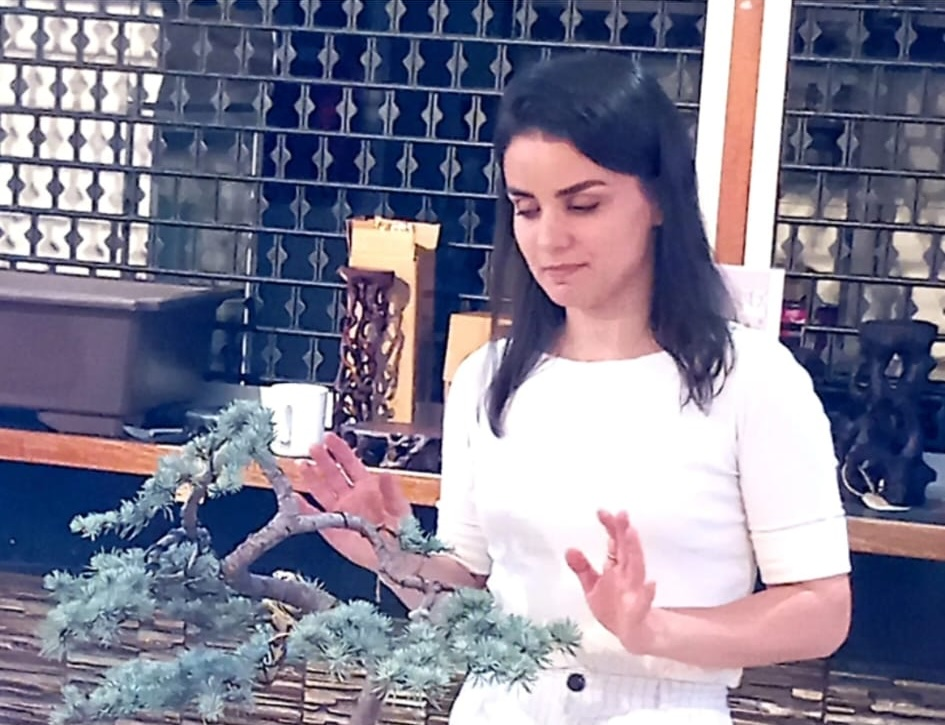
\includegraphics[angle=0,origin=c,width=1.0\textwidth]{2025_07/res/event/critique_01.jpg}
\end{minipage}\quad
\begin{minipage}[b]{.375\textwidth}
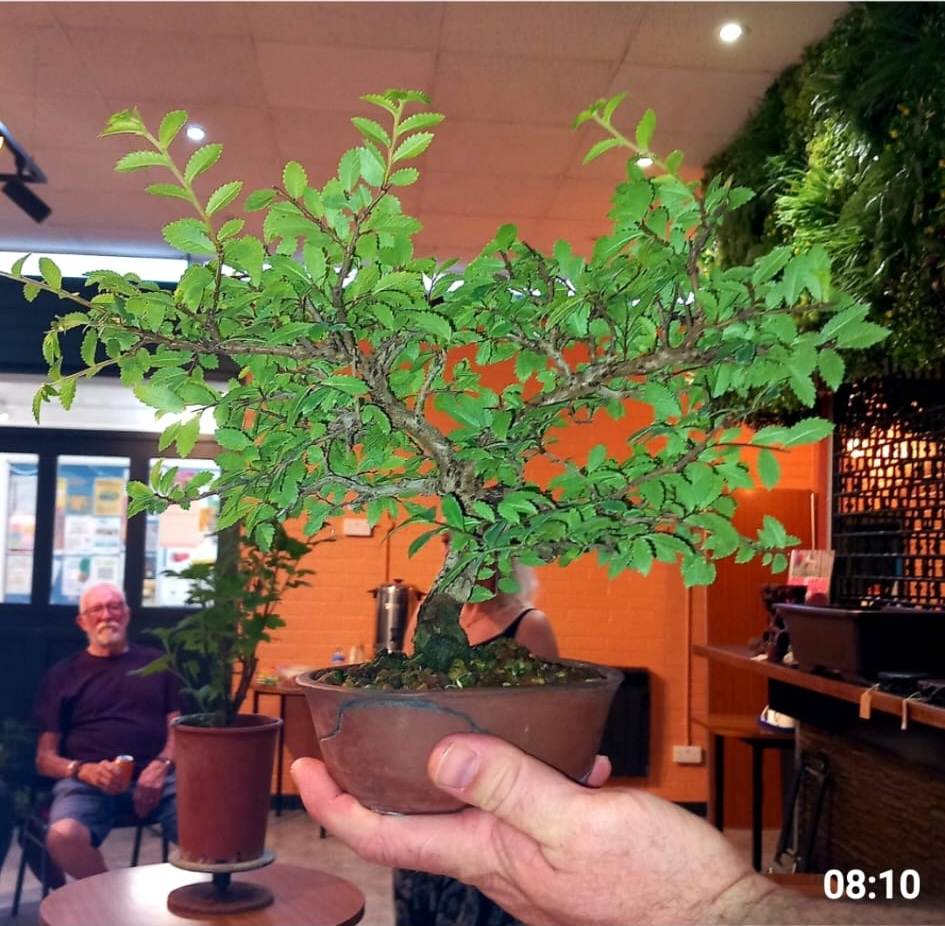
\includegraphics[angle=0,origin=c,width=1.0\textwidth]{2025_07/res/event/critique_02.jpg}
\end{minipage}

\medskip
\begin{minipage}[b]{.55\textwidth}
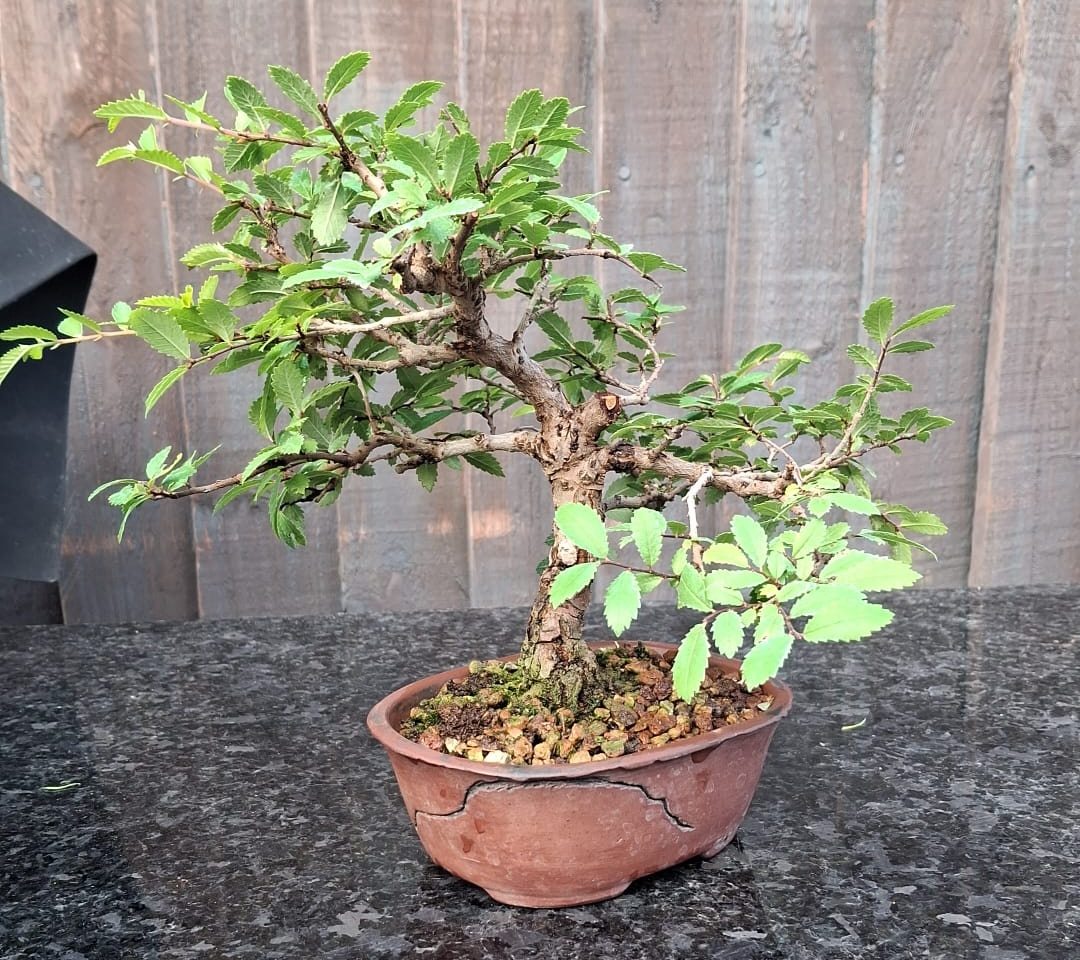
\includegraphics[angle=0,origin=c,width=1.0\textwidth]{2025_07/res/event/critique_03.jpg}
\end{minipage}\quad
\begin{minipage}[b]{.315\textwidth}
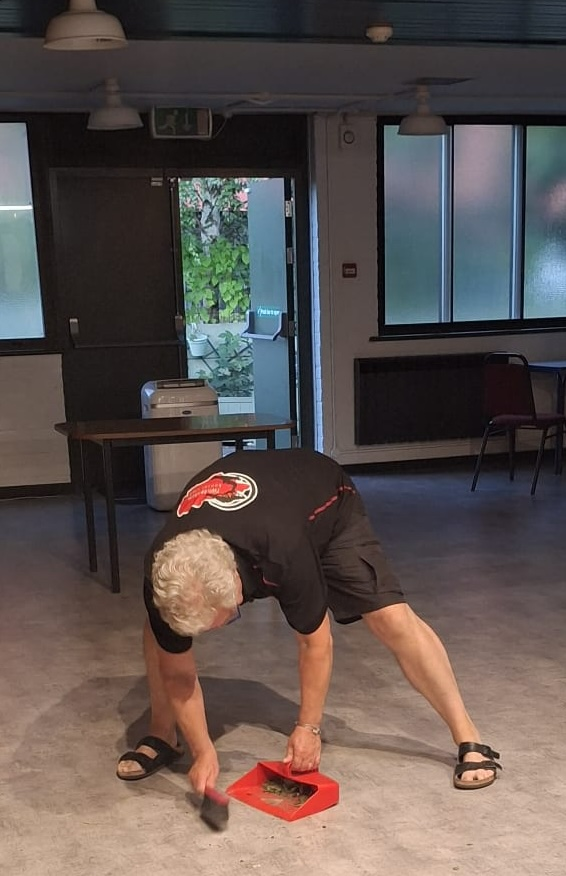
\includegraphics[angle=0,origin=c,width=1.0\textwidth]{2025_07/res/event/critique_04.jpg}
\end{minipage}

\vspace{-0.5em}
\medskip
\emph{Bonsai critique on Tina Todd's Elm (before \& after), and Tony Ulatowski's closing Tai Chi demonstration.}
\end{center}

\clearpage
\begin{multicols}{2}
